\subsubsection{Electrical Signal Standards}

The Eurorack format defines three distinct signal types that circulate between 
modules \cite{TechnicalDetailsA100}:

\begin{description}
	\item[Audio signals] Produced by sound source modules such as oscillators and noise generators. 
	Audio signals typically operate at \SI{10}{V_{pp}} ($\pm\qty{5}{V}$).
	
	\item[Control voltages (CV)] Produced by modulation sources such as LFOs and envelope generators. 
	CV signals typically range from \qty{-2.5}{V} to \qty{+2.5}{V} for LFOs, and from \qty{0}{V} to \qty{+8}{V} for envelope generators. 
	The V/Oct pitch standard is a specific application of CV, where each \qty{1}{V} increase corresponds to one octave of pitch change.
	
	\item[Gate and trigger signals] Rectangle-shaped signals used to start or 
	trigger events. 
	Gate signals are typically \qty{0}{V}/\qty{+5}{V}, though any voltage above \qty{+3}{V} is treated as logic high. 
	Only signals with sharp rising edges are suitable — slowly rising waveforms such as sine or triangle waves are not appropriate as gate or trigger sources.
\end{description}

\paragraph{Power Supply}

\begin{wrapfigure}{r}{0.32\textwidth}
	\centering
	\vspace{-1em}
	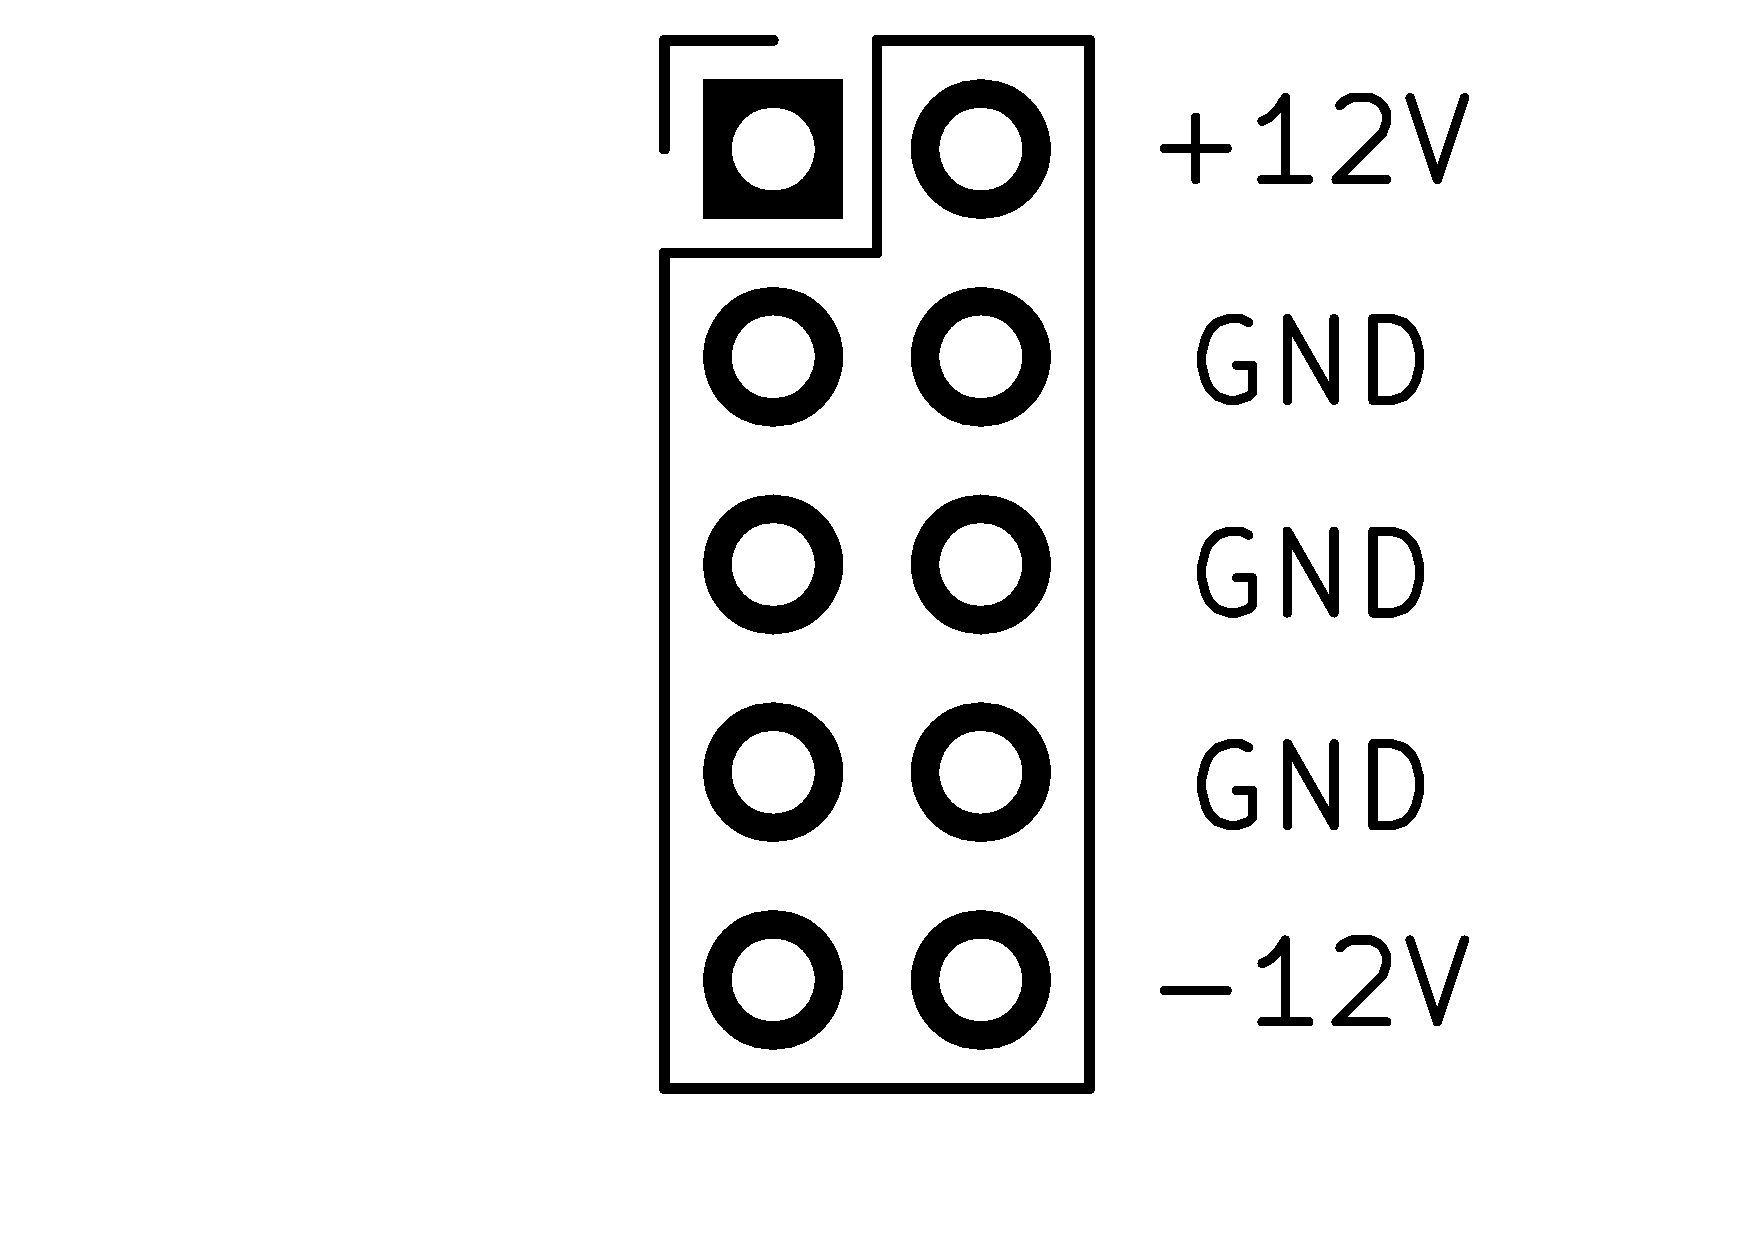
\includegraphics[width=0.3\textwidth]{../images/eurorack_fundamentals/eurorack_power_connector_fp.pdf}
	\vspace{-0.9em}
	\caption{Eurorack Power Connector Footprint with Pin Rail Assignments}
	\vspace{-1.6em}
	\label{fig:eurorack_power_connector}
\end{wrapfigure}

Eurorack modules are powered via a 10-pin ribbon cable connected to a bus board with 16-pin connectors inside the rack. 
The connectors utilize the standard \qty{2.54}{mm} pitch. 
To prevent accidental reverse insertion of the power connector it is strongly advised to use keyed (polarised) connectors with a mechanical key notch on the module side, ensuring the cable can only be inserted in the correct orientation.

The bus supplies \qty{+12}{V} and \qty{-12}{V} to all modules, with an optional \qty{+5}{V} rail for modules that require it. 

The \qty{-12}{V} line is identified by a red stripe on the ribbon cable, which must always be oriented toward the bottom of the bus connector. \cite{TechnicalDetailsA100}

\subsubsection{Eurorack Mechanical Format}


The Eurorack format defines strict mechanical constraints for all module panels.
Panel height is fixed at \qty{128.5}{mm}, derived from the 3U rack standard ($3 \times \qty{44.45}{mm} = \qty{133.4}{mm}$) minus the clearance required for the mounting rails. 
Panel width is measured in HP (horizontal pitch), where $1\,\text{HP} = \qty{5.08}{mm}$. 
Modules are mounted using M3 oval-head screws(DIN\,7985). 
These mechanical dimensions were established by Doepfer with the introduction of the A-100 system — the first Eurorack format synthesizer — and have since been adopted as the de facto standard across the modular synthesis industry \cite{ConstructionDetailsA100}.